\chapter{Взаємодія матеріальних характеристик і геометрії тріщини}
\label{ch:feedback}

У розділах~\ref{ch:fixed-crack} і~\ref{ch:ring-placement} матеріальний ефект досліджено за заданих геометрій. Така постановка дозволяє встановити прямий вплив неоднорідності, але не враховує того, що в процесі розвитку тріщини матеріал визначає її напрямок, а нова геометрія змінює наступний пружний розв'язок. У цьому розділі розмежуємо ці впливи. Задача полягає не у визначенні незалежних фізичних причин, а в контрольованому порівнянні пружних розв'язків для матеріалу та геометрії, які можна задавати окремо, хоча під час побудови траєкторії вони пов'язані.

\section{Зворотний зв'язок і факторний план}
\label{sec:feedback-design}

Позначимо через $\Gamma_{X,n}$ ламану тріщину в матеріалі $X$ після $n$ умовних приростів, через $\varphi_{X,n}$ кут дотичної її останнього відрізка, а через $\theta_{X,n}$ локальний кут МКН. На спільній початковій геометрії $\Gamma_{X,0}=\Gamma_{\mathrm H,0}$ матеріал уже змінює КІН. Наступна геометрія визначається співвідношенням~\eqref{eq:problem-step}. У позначеннях операторів цей зворотний зв'язок можна подати як
\begin{equation}
 (X,\Gamma_{X,n})\longmapsto
 (\KI,\KII)_{X,n}\longmapsto\theta_{X,n}
 \longmapsto \Gamma_{X,n+1}.
 \label{eq:feedback-map}
\end{equation}
Порівнюємо стани за однакової довжини $s$, а не за однакових координат вершини. Умовні прирости однакові за довжиною; ні час, ні критичне навантаження не визначаються.

Для довільної архітектури $X$ і величини $Q$ (наприклад $G$ або $\KI$) утворимо чотири конфігурації:
\begin{equation}
 \begin{array}{c|cc}
 &\Gamma_{\mathrm H}&\Gamma_X\\ \hline
 \mathrm H & Q_{\mathrm{HH}} & Q_{\mathrm{HX}}\\
 X & Q_{\mathrm{XH}} & Q_{\mathrm{XX}}
 \end{array}
 \label{eq:feedback-factorial}
\end{equation}
Перший індекс означає матеріал, другий --- геометрію. Діагональні розв'язки належать власним траєкторіям, позадіагональні --- контрольним задачам. Зокрема, $\Gamma_X$ в однорідному матеріалі є заданою геометрією, а не траєкторією, яку однорідне тіло самостійно вибрало за критерієм МКН.

Якщо $Q_{\mathrm{HH}}>0$, введемо нормований розклад
\begin{equation}
 \begin{aligned}
 F_{\mathrm m}&=(Q_{\mathrm{XH}}-Q_{\mathrm{HH}})/Q_{\mathrm{HH}},\\
 F_{\mathrm p}&=(Q_{\mathrm{HX}}-Q_{\mathrm{HH}})/Q_{\mathrm{HH}},\\
 F_{\mathrm i}&=(Q_{\mathrm{XX}}-Q_{\mathrm{XH}}-
                  Q_{\mathrm{HX}}+Q_{\mathrm{HH}})/Q_{\mathrm{HH}},\\
 F_{\mathrm{tot}}&=F_{\mathrm m}+F_{\mathrm p}+F_{\mathrm i}.
 \end{aligned}
 \label{eq:feedback-additive}
\end{equation}
Тут $F_{\mathrm m}$ --- прямий матеріальний внесок на однорідній геометрії; $F_{\mathrm p}$ --- внесок геометрії в однорідному матеріалі; $F_{\mathrm i}$ --- перехресна різниця (зміна матеріального внеску внаслідок заміни геометрії). Останній член не слід ототожнювати з міжкільцевими взаємодіями розділу~\ref{ch:ring-placement}. Для локального кута використовуємо абсолютні різниці в градусах, тобто ті самі чисельники без ділення. Для другого КІН нормуємо всі чотири значення на одну опорну норму $K_0=[K_{\mathrm I,HH}^2+K_{\mathrm{II},HH}^2]^{1/2}$, а потім беремо їхні різниці. Таке нормування не вироджується поблизу чистої моди I.

Часто є лише три з чотирьох розв'язків. У такому разі можна встановити лише послідовний внесок заміни геометрії в матеріалі $X$:
\begin{equation}
 F_{\mathrm p}+F_{\mathrm i}
 =\frac{Q_{\mathrm{XX}}-Q_{\mathrm{XH}}}{Q_{\mathrm{HH}}}.
 \label{eq:feedback-sequential}
\end{equation}
Якщо всі $Q$ додатні, той самий облік можна записати через відношення
\begin{equation}
 R_{\mathrm{dir}}=\frac{Q_{\mathrm{XH}}}{Q_{\mathrm{HH}}},
 \quad R_{\mathrm{seq}}=\frac{Q_{\mathrm{XX}}}{Q_{\mathrm{XH}}},
 \quad R_{\mathrm{tot}}=R_{\mathrm{dir}}R_{\mathrm{seq}}.
 \label{eq:feedback-ratio}
\end{equation}
У цьому записі $R_{\mathrm{seq}}$ не є чистим геометричним відношенням $Q_{\mathrm{HX}}/Q_{\mathrm{HH}}$. Це важлива відмінність ранніх серій від повного факторного плану.

\section{Перші власні траєкторії: одночасна активація трьох кілець}
\label{sec:feedback-m3}

Після розрахунків із замороженою тріщиною вперше виконано незалежне продовження однорідної, трьох м'яких та трьох жорстких кілець на два прирости по 4 мм. Конфігурації цієї ранньої серії M3 не збігаються з soft1, soft2 і stiff13. Результати дають змогу визначити послідовний, але не чистий геометричний внесок.

\begin{table}[htbp]
 \centering
 \caption{Послідовний розклад $G$ для трьох однаково активованих кілець (вихідне сімейство сіток). Останній стовпець --- відсоткові пункти.}
 \label{tab:feedback-m3}
 \begin{tabular}{lrrrr}
 \toprule
 Конфігурація / стан & $R_{\mathrm{dir}}$ & $R_{\mathrm{seq}}$ & $R_{\mathrm{tot}}$ & $100(F_{\mathrm p}+F_{\mathrm i})$\\
 \midrule
М'які / S1 & $1,006199$ & $0,999511$ & $1,005706$ & $-0,0492$ \\
М'які / S2 & $1,021813$ & $0,998826$ & $1,020614$ & $-0,1199$ \\
Жорсткі / S1 & $0,981870$ & $1,000396$ & $0,982259$ & $+0,0389$ \\
Жорсткі / S2 & $0,970687$ & $1,000813$ & $0,971476$ & $+0,0789$ \\

 \bottomrule
 \end{tabular}
\end{table}

На S0 геометрія спільна, тому $R_{\mathrm{seq}}=1$. Після двох приростів для м'яких кілець заміна геометрії в тому самому матеріалі послаблює підсилення, а для жорстких послаблює екранування. Обидва ефекти малі порівняно з прямим внеском. Знак енергетичного контрасту м'яких кілець, розглянутий у розділі~\ref{ch:fixed-crack}, змінюється і на власній траєкторії. Усі ненульові відношення розрізняються за первинним критерієм M3, але не за консервативним.

\begin{figure}[htbp]
 \centering
 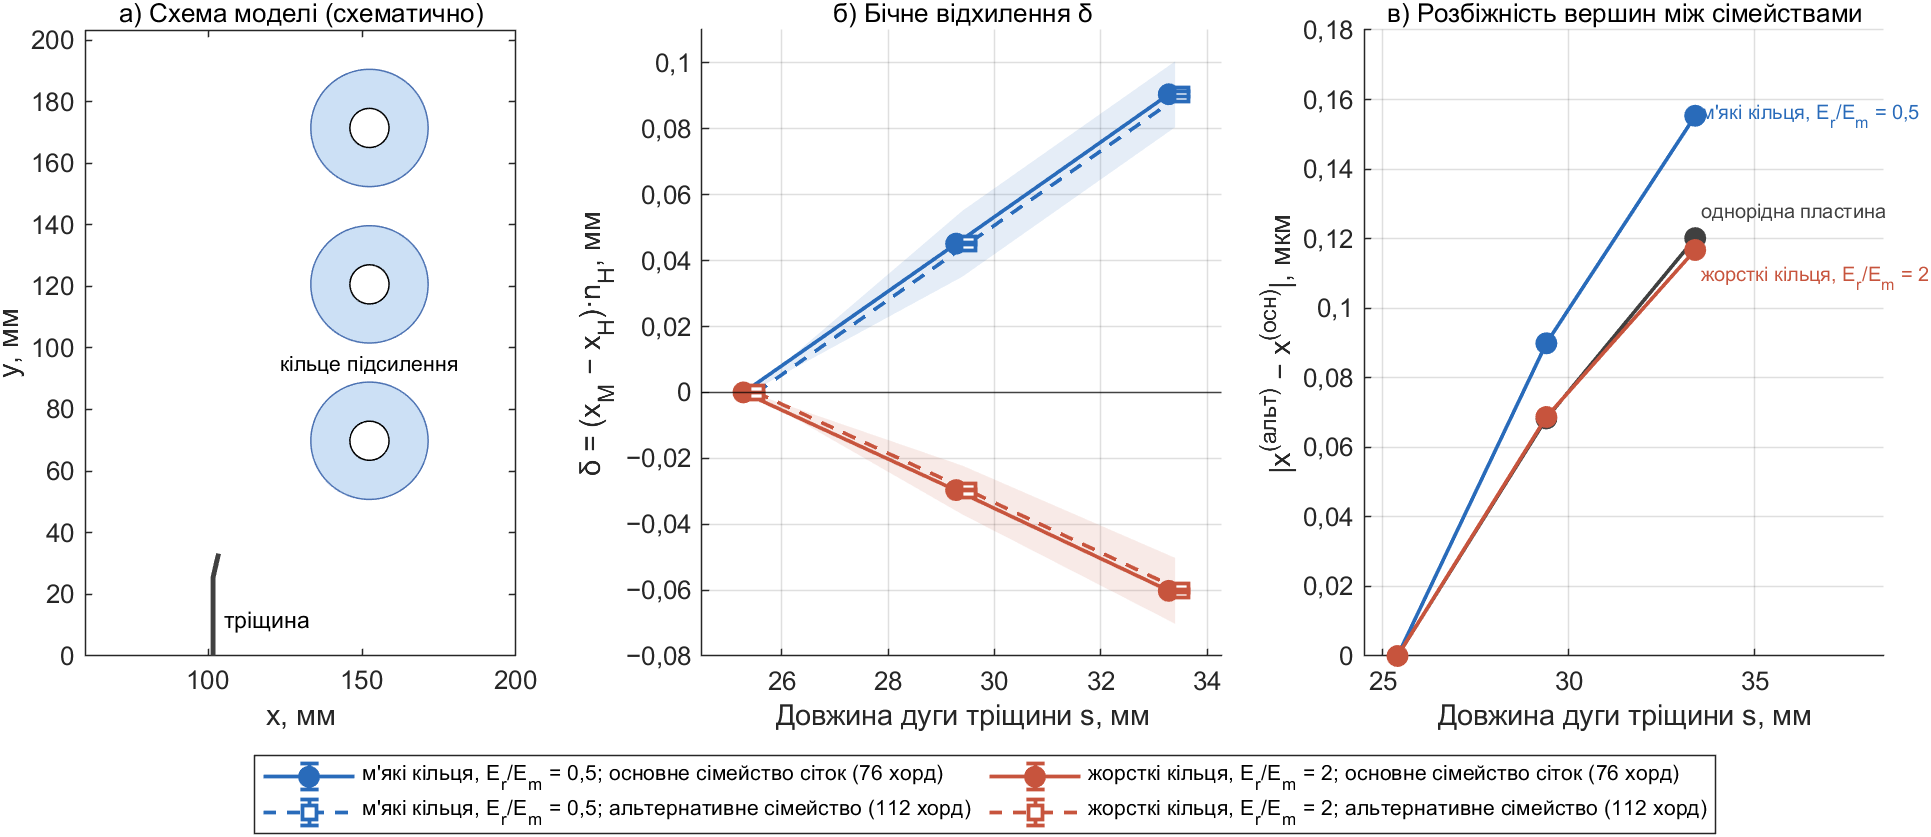
\includegraphics[width=\textwidth]{figures/m4a_fig1_paths.png}
 \caption{Порівняння двокрокових траєкторій із трьома активними кільцями на двох зовнішніх сімействах сіток. Бічні відхилення та міжсіткову розбіжність наведено окремо.}
 \label{fig:feedback-m4a-paths}
\end{figure}

\begin{figure}[htbp]
 \centering
 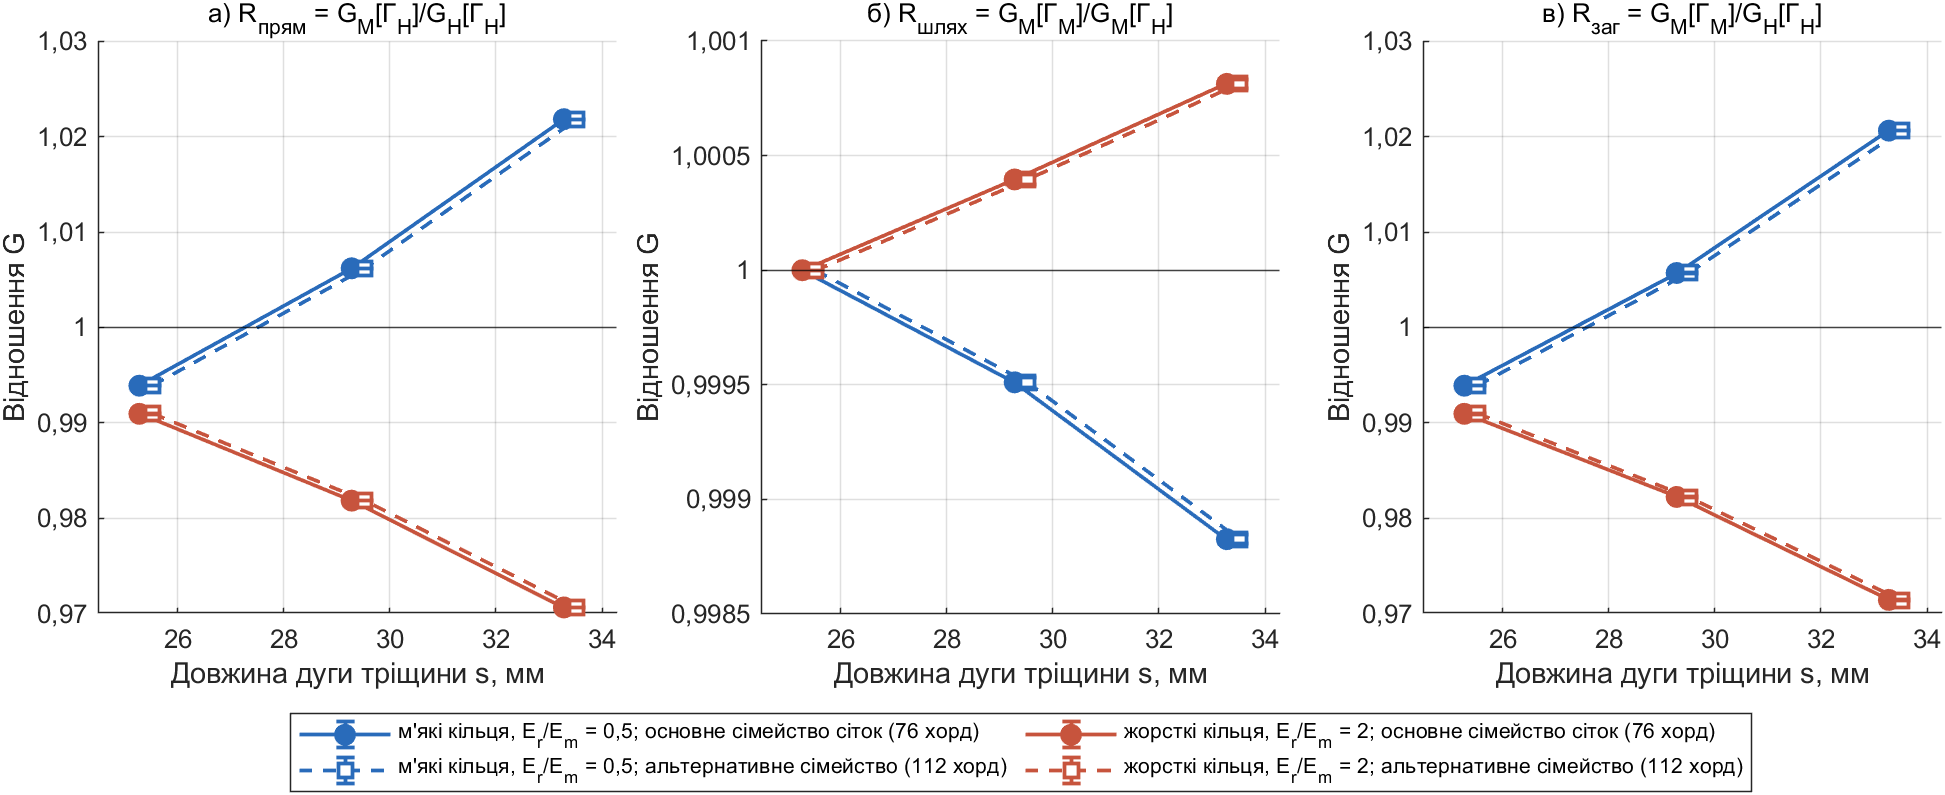
\includegraphics[width=\textwidth]{figures/m4a_fig2_ratios.png}
 \caption{Відношення прямого, послідовного та повного ефектів для двох сімейств сіток. Смуги відповідають первинному індикатору, а не гарантованій похибці.}
 \label{fig:feedback-m4a-ratios}
\end{figure}

Для цих коротких траєкторій у M4.A незалежно повторено весь двокроковий розрахунок на альтернативному сімействі зовнішніх сіток із 112 хордами замість 76, зберігаючи привершинне ядро. На S2 для м'яких кілець $R_{\mathrm{seq}}$ становить 0,998826 на обох сімействах із точністю до шести знаків, для жорстких --- 1,000813. Бічне зміщення відносно однорідного шляху становить відповідно $+0{,}09050$ та $-0{,}06022$ мм; заміна сімейства змінює його на $3{,}5\cdot10^{-5}$ та $-3{,}4\cdot10^{-6}$ мм. Таким чином, підтверджено стійкість саме двокрокового спостереження до однієї конкретної зміни зовнішньої дискретизації. Дослідження не охоплює локального подрібнення ядра, зменшення приросту $\Delta a$ чи довших траєкторій.

\section{Прямий та повний ефекти вибраних архітектур на S0--S4}
\label{sec:feedback-existing}

Для архітектур, вибраних у розділі~\ref{ch:ring-placement}, незалежно побудовано чотири власні траєкторії до S4. На S0 усі 23 поля масивів сіток збігаються; різні SHA сирих MAT-файлів пояснюються відмінністю метаданих. Отже, на S0 прямий та повний ефекти збігаються на рівні дискретного розв'язку. На S2 доступні прямі розрахунки M4.B, а також власні LP1/A0. Однорідні опорні значення $G$ цих історичних серій відрізняються приблизно на $8\cdot10^{-8}$ відносно одне одного; тому зіставлення їхніх нормованих контрастів є наближеним міжсерійним порівнянням, а не точною тотожністю чотирьох записів однієї кампанії.

\begin{table}[htbp]
 \centering
 \caption{Прямі та повні контрасти $G$ вибраних архітектур, \%. Стовпець залишку --- відсоткові пункти.}
 \label{tab:feedback-s2}
 \begin{tabular}{lrrrr}
 \toprule
 & S0 & \multicolumn{3}{c}{S2}\\
 \cmidrule(lr){3-5}
 Архітектура & $F_{\mathrm{tot}}=F_{\mathrm m}$ & $F_{\mathrm m}$ & $F_{\mathrm{tot}}$ & $F_{\mathrm p}+F_{\mathrm i}$\\
 \midrule
stiff13 & $-3,9312$ & $-5,4780$ & $-5,3478$ & $+0,1301$ \\
soft2 & $-4,2590$ & $-3,6278$ & $-3,5768$ & $+0,0510$ \\
soft1 & $+2,7458$ & $+4,4298$ & $+4,2395$ & $-0,1903$ \\

 \bottomrule
 \end{tabular}
\end{table}

Для всіх трьох архітектур на S2 залишок протилежний прямому ефекту. Відсутні розрахунки $\mathrm H$ на $\Gamma_X$, тому окремо встановити знак $F_{\mathrm p}$ та $F_{\mathrm i}$ на S2 неможливо. Перші спостереження мотивували наступний розрахунковий експеримент на S4.

\begin{figure}[htbp]
 \centering
 \begin{tikzpicture}[x=1mm,y=1mm,font=\small]
 \draw[->] (0,0)--(121,0) node[right] {$s$, мм};
 \draw[->] (0,-42)--(0,42) node[above] {$F_G$, \%};
 \foreach \v in {-8,-6,-4,-2,2,4,6,8}{
  \draw[black!15] (0,5*\v)--(112,5*\v);
  \node[anchor=east,font=\scriptsize] at (-1,5*\v) {\v};
 }
 \foreach \i/\s in {0/25,1/29,2/33,3/37,4/41}{
  \draw (10+24*\i,0)--(10+24*\i,-1);
  \node[anchor=north,font=\scriptsize] at (10+24*\i,-43) {S\i};
 }
\draw[red!65!black,line width=.8pt] (10,-19.65607)--(34,-22.48607)--(58,-26.73923)--(82,-31.20558)--(106,-35.86585);
\draw[red!65!black,fill=white] (10,-19.65607) circle[radius=.8mm];
\draw[red!65!black,fill=white] (34,-22.48607) circle[radius=.8mm];
\draw[red!65!black,fill=white] (58,-26.73923) circle[radius=.8mm];
\draw[red!65!black,fill=white] (82,-31.20558) circle[radius=.8mm];
\draw[red!65!black,fill=white] (106,-35.86585) circle[radius=.8mm];
\fill[red!65!black] (10,-19.65607) circle[radius=1mm];
\fill[red!65!black] (58,-27.38978) circle[radius=1mm];
\fill[red!65!black] (106,-36.84178) circle[radius=1mm];
\node[anchor=west,font=\scriptsize,text=red!65!black] at (112,-36.84178) {stiff13};
\draw[blue!65!black,line width=.8pt] (10,-21.29476)--(34,-19.40687)--(58,-17.88408)--(82,-16.29774)--(106,-14.65908);
\draw[blue!65!black,fill=white] (10,-21.29476) circle[radius=.8mm];
\draw[blue!65!black,fill=white] (34,-19.40687) circle[radius=.8mm];
\draw[blue!65!black,fill=white] (58,-17.88408) circle[radius=.8mm];
\draw[blue!65!black,fill=white] (82,-16.29774) circle[radius=.8mm];
\draw[blue!65!black,fill=white] (106,-14.65908) circle[radius=.8mm];
\fill[blue!65!black] (10,-21.29476) circle[radius=1mm];
\fill[blue!65!black] (58,-18.13920) circle[radius=1mm];
\fill[blue!65!black] (106,-15.15980) circle[radius=1mm];
\node[anchor=west,font=\scriptsize,text=blue!65!black] at (112,-15.15980) {soft2};
\draw[green!45!black,line width=.8pt] (10,13.72911)--(34,16.37179)--(58,21.19736)--(82,26.29237)--(106,31.64468);
\draw[green!45!black,fill=white] (10,13.72911) circle[radius=.8mm];
\draw[green!45!black,fill=white] (34,16.37179) circle[radius=.8mm];
\draw[green!45!black,fill=white] (58,21.19736) circle[radius=.8mm];
\draw[green!45!black,fill=white] (82,26.29237) circle[radius=.8mm];
\draw[green!45!black,fill=white] (106,31.64468) circle[radius=.8mm];
\fill[green!45!black] (10,13.72911) circle[radius=1mm];
\fill[green!45!black] (58,22.14903) circle[radius=1mm];
\fill[green!45!black] (106,33.45580) circle[radius=1mm];
\node[anchor=west,font=\scriptsize,text=green!45!black] at (112,33.45580) {soft1};
 \node[anchor=west,font=\scriptsize] at (1,-50) {Порожні: власна траєкторія B0; заповнені: фіксована геометрія.};
 \node[anchor=west,font=\scriptsize] at (1,-55) {S4: прямий ефект B9, решта станів --- базові сітки.};
 \node[anchor=west,font=\scriptsize] at (1,-60) {Довжини S0--S4: 25,4; 29,4; 33,4; 37,4; 41,4 мм.};
\end{tikzpicture}

 \caption{Повні енергетичні контрасти власних траєкторій та прямі матеріальні контрасти у вибраних станах. Значення S4 для прямого ефекту отримано в кампанії X6 на B9; лінії з'єднують повні контрасти на базовій дискретизації B0, не є інтерполяцією прямого ефекту.}
 \label{fig:feedback-direct-total}
\end{figure}

\section{Шість перехресних розрахунків S4}
\label{sec:feedback-x6}

Для повного факторного плану на $s=41{,}4$ мм використано чотири збережені геометрії та відповідні сітки локального рівня B9 з дослідження A1. Діагональні розв'язки не перераховували. Для кожної архітектури виконано дві задачі: матеріал $X$ на сітці $\Gamma_{\mathrm H}$ та однорідний матеріал на сітці $\Gamma_X$. Усередині кожної геометрії сітка не змінювалася. Усі шість задач пройшли 16 критеріїв визначення КІН, окремі перевірки фаз та відповідності матеріальної конфігурації. Повторне читання записів підтвердило їхню цілісність без нових розв'язків. Наукове приймання стосується саме цих шести задач, а не інших станів траєкторії.

\begin{table}[htbp]
 \centering
 \caption{Чотири енергетичні значення факторного плану S4 на B9, в одиницях $10^{-8}$ Н/мм при силі 1 Н.}
 \label{tab:feedback-cross}
 \begin{tabular}{lrrrr}
 \toprule
 Архітектура & $G_{\mathrm{HH}}$ & $G_{\mathrm{XH}}$ & $G_{\mathrm{HX}}$ & $G_{\mathrm{XX}}$\\
 \midrule
stiff13 & $1,539127$ & $1,425719$ & $1,542243$ & $1,428716$ \\
soft2 & $1,539127$ & $1,492461$ & $1,540581$ & $1,494004$ \\
soft1 & $1,539127$ & $1,642112$ & $1,533379$ & $1,636545$ \\

 \bottomrule
 \end{tabular}
\end{table}

\begin{table}[htbp]
 \centering
 \caption{Розклад енергетичного контрасту на S4, \%. Останній стовпець --- частка прямого ефекту, компенсована зміною геометрії: $\rho_{\mathrm c}=-100(F_{\mathrm p}+F_{\mathrm i})/F_{\mathrm m}$.}
 \label{tab:feedback-G}
 \begin{tabular}{lrrrrr}
 \toprule
 Архітектура & $F_{\mathrm m}$ & $F_{\mathrm p}$ & $F_{\mathrm i}$ & $F_{\mathrm{tot}}$ & $\rho_{\mathrm c}$\\
 \midrule
stiff13 & $-7,3684$ & $+0,2024$ & $-0,0077$ & $-7,1736$ & $2,64$ \\
soft2 & $-3,0320$ & $+0,0945$ & $+0,0058$ & $-2,9317$ & $3,31$ \\
soft1 & $+6,6912$ & $-0,3735$ & $+0,0117$ & $+6,3294$ & $5,41$ \\

 \bottomrule
 \end{tabular}
\end{table}

\begin{figure}[htbp]
 \centering
 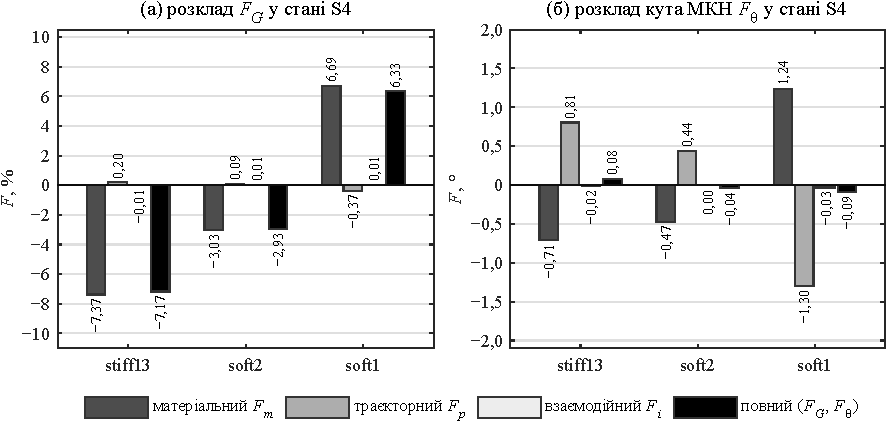
\includegraphics[width=\textwidth]{figures/F07_1_rozklad_S4.pdf}
 \caption{Розклад енергетичного контрасту та зміни локального кута МКН на S4 (B9). Шкали двох панелей різні; усі внески відраховано від стану H на однорідній геометрії.}
 \label{fig:feedback-x6}
\end{figure}

На S4 матеріальний внесок становить 102,7; 103,4 та 105,7\,\% від модуля відповідного повного енергетичного контрасту. Внесок геометрії має протилежний знак у всіх трьох архітектурах. Взаємодія набагато менша за два основні внески, її знак не є однаковим. Заміна геометрії в матеріалі архітектури компенсує приблизно 2,6--5,4\,\% прямого ефекту. Застосування такого самого розкладу до $J$ дає близькі результати (найбільша абсолютна відмінність окремого члена розкладу від розкладу $G$ менша за $2\cdot10^{-6}$ у безрозмірній шкалі).

Перехресні внески обчислено на одному рівні B9. Раніше спостережена зміна енергетичного контрасту при заміні сімейства на S2 ($U_m=3{,}1\cdot10^{-5}$) є лише орієнтиром. Навіть якщо $|F_{\mathrm i}|>2U_m$, з цього не випливає розрізнення взаємодії на S4. Для soft2 $|F_{\mathrm i}|$ менше $2U_m$. Локальне подрібнення діагональних розв'язків A1 не визначає похибки перехресних задач. Консервативну класифікацію soft2 для повного ефекту на власній траєкторії залишено без змін.

\subsection{Залежність від опорного стану та шкали}

Розклад~\eqref{eq:feedback-additive} точний, але залежить від опорної конфігурації. Якщо визначати матеріальний внесок на геометрії $\Gamma_X$ (за того самого нормування на $Q_{\mathrm{HH}}$), він становитиме $F_{\mathrm m}+F_{\mathrm i}$. Симетричний спосіб розподілу взаємодії між матеріалом і геометрією дає
\begin{equation}
 \Phi_{\mathrm m}=F_{\mathrm m}+\tfrac12 F_{\mathrm i},
 \quad \Phi_{\mathrm p}=F_{\mathrm p}+\tfrac12 F_{\mathrm i}.
 \label{eq:feedback-shapley}
\end{equation}
Їхня сума дорівнює повному ефекту. Для додатних $Q$ можливий також мультиплікативний облік:
\begin{equation}
 R_{\mathrm m}=\frac{Q_{\mathrm{XH}}}{Q_{\mathrm{HH}}},
 \quad R_{\mathrm p}=\frac{Q_{\mathrm{HX}}}{Q_{\mathrm{HH}}},
 \quad R_{\mathrm i}=\frac{Q_{\mathrm{XX}}Q_{\mathrm{HH}}}
 {Q_{\mathrm{XH}}Q_{\mathrm{HX}}},
 \quad R_{\mathrm{tot}}=R_{\mathrm m}R_{\mathrm p}R_{\mathrm i}.
 \label{eq:feedback-mult}
\end{equation}
Тут $R_{\mathrm i}$ не дорівнює $1+F_{\mathrm i}$, оскільки множення основних відношень уже містить перехресний добуток. Для енергетичних даних S4 зміна матеріального внеску при переході від $\Gamma_{\mathrm H}$ до $\Gamma_X$ не перевищує 0,012 відсоткового пункта. Тому висновки про домінування прямого внеску та його часткову компенсацію стійкі до цих конкретних способів обліку. Проте жоден не є єдиним фізичним поділом: геометрія $\Gamma_X$ сама виникла внаслідок дії матеріалу на попередніх кроках.

\section{Напрямні ефекти та геометрична пам'ять}
\label{sec:feedback-direction}

Для КІН моди I отримуємо подібний до $G$ характер розкладу. Для КІН моди II та локального кута МКН, навпаки, два основні внески майже компенсуються (табл.~\ref{tab:feedback-angle}). Тут усі $K_{\mathrm{II}}$ нормовано на одну й ту саму опорну норму $K_0$; не йдеться про відношення до власної норми КІН кожної задачі.

\begin{table}[htbp]
 \centering
 \caption{Розклади зміни КІН і локального кута МКН на S4. Нормування зазначено в першому стовпці.}
 \label{tab:feedback-angle}
 \small
 \begin{tabular}{lrrrr}
 \toprule
 Архітектура / величина & Матеріал & Геометрія & Взаємодія & Разом\\
 \midrule
stiff13 / $K_{\mathrm I}$, \% & $-3,7650$ & $+0,1087$ & $+0,0037$ & $-3,6526$ \\
stiff13 / $K_{\mathrm{II}}/K_0$ & $+0,005450$ & $-0,007028$ & $+0,000404$ & $-0,001175$ \\
stiff13 / $\theta$, град & $-0,7113$ & $+0,8057$ & $-0,0166$ & $+0,0778$ \\
soft2 / $K_{\mathrm I}$, \% & $-1,5343$ & $+0,0519$ & $+0,0051$ & $-1,4772$ \\
soft2 / $K_{\mathrm{II}}/K_0$ & $+0,003839$ & $-0,003827$ & $+0,000084$ & $+0,000097$ \\
soft2 / $\theta$, град & $-0,4714$ & $+0,4387$ & $-0,0030$ & $-0,0357$ \\
soft1 / $K_{\mathrm I}$, \% & $+3,3013$ & $-0,2094$ & $+0,0232$ & $+3,1150$ \\
soft1 / $K_{\mathrm{II}}/K_0$ & $-0,010695$ & $+0,011286$ & $+0,000652$ & $+0,001243$ \\
soft1 / $\theta$, град & $+1,2379$ & $-1,2959$ & $-0,0308$ & $-0,0888$ \\

 \bottomrule
 \end{tabular}
\end{table}

Наприклад, для soft1 матеріал на $\Gamma_{\mathrm H}$ збільшив би кут МКН на $1{,}238^\circ$, проте заміна геометрії в однорідному матеріалі зменшує його на $1{,}296^\circ$. З урахуванням взаємодії повна різниця локального кута дорівнює лише $-0{,}089^\circ$. Така компенсація не означає, що координати вершини або напрямок уже утвореної ламаної збігаються.

Дійсно, якщо $\Delta\varphi_n=\varphi_{X,n}-\varphi_{\mathrm H,n}$, а $\Delta\theta_n=\theta_{X,n}-\theta_{\mathrm H,n}$, то
\begin{equation}
 \Delta\varphi_{n+1}=\Delta\varphi_n+\Delta\theta_n,\qquad
 \Delta\varphi_n=\sum_{j=0}^{n-1}\Delta\theta_j.
 \label{eq:feedback-heading}
\end{equation}
Кут $\theta_n$ є прогнозом для наступного приросту, тому не входить до суми для вже утвореного останнього відрізка $n$. Звідси точна геометрична різниця координат
\begin{equation}
 \boldsymbol x_{X,n}-\boldsymbol x_{\mathrm H,n}
 =\Delta a\sum_{k=1}^{n}
 [\boldsymbol\tau(\varphi_{X,k})-\boldsymbol\tau(\varphi_{\mathrm H,k})].
 \label{eq:feedback-tip-sum}
\end{equation}
Проєктуючи на нормаль $\boldsymbol n_{\mathrm H,n}$ та лінеаризуючи за малими різницями кутів у радіанах, отримуємо
\begin{equation}
 d_n=\Delta a\sum_{k=1}^{n}
 \Delta\varphi_k\cos(\varphi_{\mathrm H,k}-\varphi_{\mathrm H,n})
 +O\!\left(\Delta a\sum_{k=1}^{n}|\Delta\varphi_k|^2\right).
 \label{eq:feedback-lateral}
\end{equation}
Таким чином, навіть якщо $\Delta\theta_n$ стає малим, попередні різниці кутів залишаються в $\Delta\varphi_k$ та накопиченому зміщенні $d_n$. Для майже паралельних коротких шляхів і приблизно сталої різниці напрямків після першого приросту маємо грубу оцінку $d_n\simeq n\Delta a\sin(\Delta\theta_0)$. Це не твердження про те, що матеріал діє лише на першому кроці.

\begin{figure}[htbp]
 \centering
 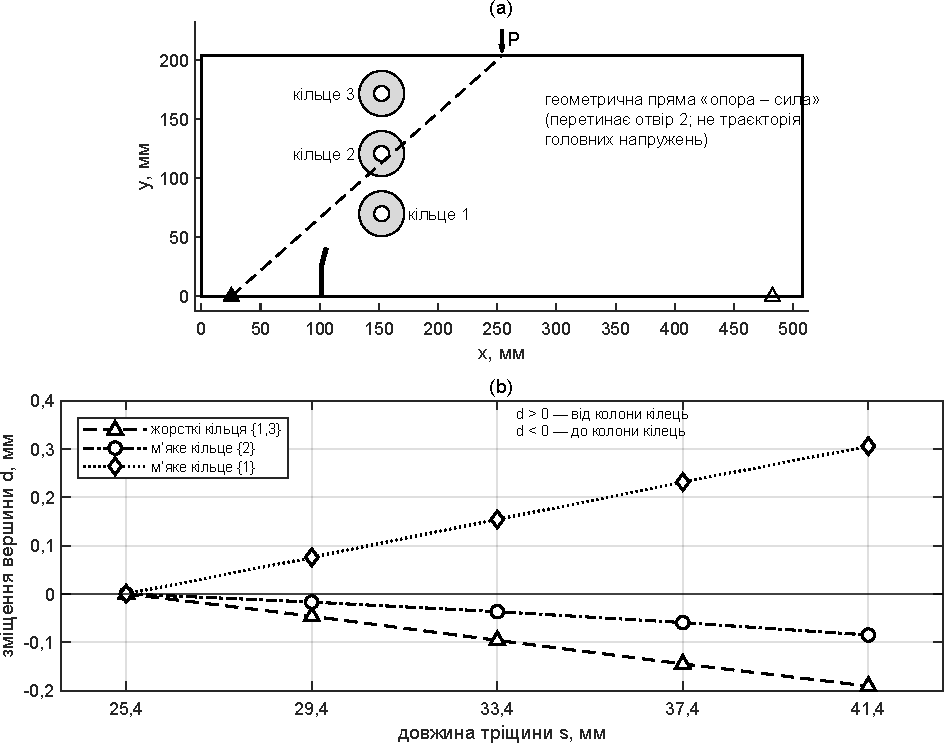
\includegraphics[width=\textwidth]{figures/M5_1_geometriia_UA.pdf}
 \caption{Однорідна траєкторія до S4 і бічні зміщення вибраних архітектур. Пряма опора--сила є геометричним орієнтиром.}
 \label{fig:feedback-offset}
\end{figure}

\begin{table}[htbp]
 \centering
 \caption{Різниці кутів і бічні зміщення на власних траєкторіях S4 (B0). Останній стовпець --- відношення грубої оцінки першого зламу до фактичного зміщення $\rho_1=16\sin\Delta\theta_0/d_4$.}
 \label{tab:feedback-heading}
 \begin{tabular}{lrrrrr}
 \toprule
 & $\Delta\theta_0$, град & $\Delta\varphi_4$, град & $\Delta\theta_4$, град & $d_4$, мм & $\rho_1$\\
 \midrule
stiff13 & $-0,6627$ & $-0,6611$ & $+0,0778$ & $-0,1909$ & $0,969$ \\
soft2 & $-0,2433$ & $-0,3669$ & $-0,0356$ & $-0,0852$ & $0,798$ \\
soft1 & $+1,0842$ & $+1,0682$ & $-0,0888$ & $+0,3057$ & $0,990$ \\

 \bottomrule
 \end{tabular}
\end{table}

Незалежне відновлення координат за~\eqref{eq:feedback-tip-sum} для 12 пар станів S1--S4 дає максимальну розбіжність менше $10^{-12}$ мм, а накопичених кутів за~\eqref{eq:feedback-heading} --- менше $10^{-12}$ градуса. Лінеаризація~\eqref{eq:feedback-lateral} відтворює бічне зміщення з максимальною абсолютною розбіжністю менше $10^{-3}$ мм у цих станах. Ці перевірки стосуються геометричної рекурсії, а не точності прогнозування фізичної траєкторії.

На S4 наближена оцінка на основі першого приросту становить 80--99\,\% фактичного бічного зміщення. Цей збіг підтверджує її придатність як геометричної оцінки для коротких шляхів, але не встановлює причинної частки першого зламу: для цього потрібні контрольні траєкторії із заданою зміною лише одного кроку. Кутова компенсація в факторному плані S4 сумісна з тенденцією до локальної моди I, але не є доведенням динамічної стійкості траєкторії.

\section{Перевірка передбачень і межі енергетичної чутливості}
\label{sec:feedback-predictions}

До виконання перехресних задач зафіксовано два основні передбачення: П1 --- модуль прямого матеріального внеску не менший за 90\,\% модуля повного ефекту; П2 --- сумарний залишок $F_{\mathrm p}+F_{\mathrm i}$ протилежний прямому внеску за знаком. Знак кожного з $F_{\mathrm p}$ та $F_{\mathrm i}$ окремо не передбачався (П3). Додаткове дослідницьке передбачення П4 переносило спостережені при S0 і S2 відношення розрахованого ефекту до першого наближення~\eqref{eq:ring-first-G} на S4. П4 не було критерієм прийняття розв'язку.

\begin{table}[htbp]
 \centering
 \caption{Перевірка дослідницького передбачення П4 для прямого ефекту S4. Перші три числові стовпці у відсотках.}
 \label{tab:feedback-p4}
 \begin{tabular}{lrrrr}
 \toprule
 Архітектура & Перше наближення & Інтервал П4 & $F_{\mathrm m}$ & Відношення\\
 \midrule
stiff13 & $-5,702$ & $-7{,}11\ldots-6{,}50$ & $-7,3684$ & $1,292$ \\
soft2 & $-4,293$ & $-3{,}28\ldots-2{,}99$ & $-3,0320$ & $0,706$ \\
soft1 & $+8,140$ & $+5{,}67\ldots+6{,}23$ & $+6,6912$ & $0,822$ \\

 \bottomrule
 \end{tabular}
\end{table}

П1 та П2 підтверджено для всіх трьох архітектур. П4 підтверджено лише для soft2, для stiff13 та soft1 отримані значення поза інтервалами. Цей результат має особливе значення: знак першого наближення правильний, але переносити коефіцієнт поправки, встановлений на коротших тріщинах, не можна без перевірки. Ще до розрахунку для stiff13 та soft1 існувала суперечність П2 і П4. Відомі повні ефекти на B9 дорівнювали $-7{,}174$ і $+6{,}329$\,\%, а за П2 при встановленому знаку прямого ефекту його модуль мав бути більшим за модуль повного. Інтервали П4 цілком лежали нижче цих модулів. Перехресний експеримент вирішив суперечність на користь П2, а не П4.

Спільна ознака двох архітектур, для яких П4 не справдилося, --- активне кільце 1, найближче до вершини. Це підстава для гіпотези, але не для висновку про причину: також можливі вплив скінченного контрасту, односторонньої різниці S3--S4, зміни напрямку та способу нормування енергетичної похідної. Для перевірки потрібні незалежні варіації контрасту і приросту тріщини. Межі П4 збережено без ретроспективного уточнення.

\section{Енергетичне тлумачення та перехід до довших траєкторій}
\label{sec:feedback-summary}

Додатково розглянемо податливість власних траєкторій. Відносний контраст $C_X/C_{\mathrm H}-1$ для stiff13 змінюється від $-0{,}76$ до $-0{,}86$\,\%, для soft2 --- від $+0{,}41$ до $+0{,}33$\,\%, для soft1 --- від $+0{,}38$ до $+0{,}46$\,\%. Різниці абсолютних податливостей $C_X-C_{\mathrm H}$ за чотири кроки мають той самий знак зміни, що й відповідний контраст $G$. Це узгоджується із~\eqref{eq:fixed-compliance-G}, але оскільки геометрії і сітки різні, а похідну замінено різницями на 4 мм, не є незалежним обчисленням прямої матеріальної чутливості.

\begin{figure}[htbp]
 \centering
 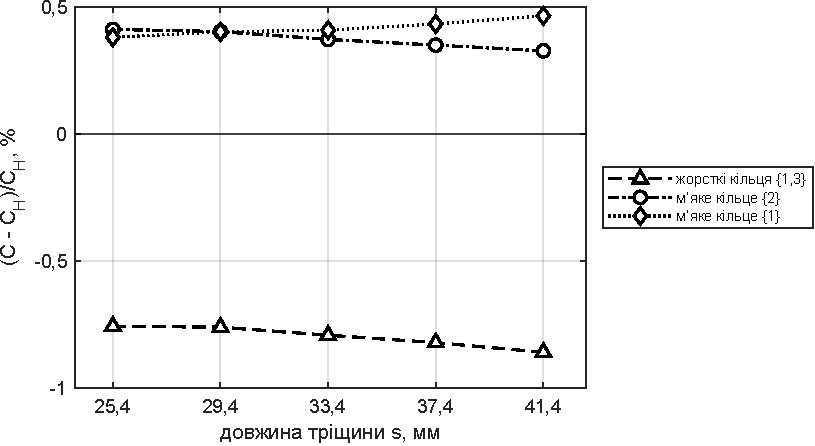
\includegraphics[width=\textwidth]{figures/M5_3_podatlyvist_UA.pdf}
 \caption{Відносна зміна податливості вздовж власних траєкторій S0--S4. Для енергетичного співвідношення потрібна похідна абсолютної різниці податливостей, а не лише відносного контрасту.}
 \label{fig:feedback-compliance}
\end{figure}

На останніх двох інтервалах розбіжність між оцінкою контрасту за різницями податливостей та середнім EDI-контрастом кінців інтервалу становить приблизно 0,03--0,5 відсоткового пункта; на початкових інтервалах розбіжність більша. Результат є додатковою діагностикою, а не новою межею похибки.

Загалом для фіксованої S4 геометрії прямий вплив матеріальної неоднорідності встановлює знак і основну величину енергетичного контрасту, а зміна геометрії частково його компенсує. Для локального кута спостерігається майже повна компенсація, проте накопичений напрямок та бічне зміщення не зникають. Перехресний план не розділяє внесок окремих змін ламаної, не встановлює чисельної похибки всіх членів та не визначає поведінку біля міжфазної межі. У наступному розділі розглянемо фактично прийняті власні траєкторії до дальших станів та їхні енергетичні й геометричні характеристики.
